% Chapter 4

\chapter{Some Elements Considered}
\label{chap:Elements}
We have derived a general finite element scheme for Lagrangian computational fluid dynamics. This general framework has made it very easy to consider a number of different mixed finite element formulations. We have only considered quadrilateral 2-D elements in this research, but the formulation is general enough to allow for triangles or even 3-D tetrahedral or hexahedral meshes. In this chapter, we analyze a wide range of bi-linear and bi-quadratic mixed finite element pairs and narrow the results down to four elements to warrant further numerical consideration. Please note that all methods use a $Q_0$ energy representation.

\section{Some Guidelines}
In his canonical textbook on the finite element method, Hughes \cite{Hughes1987} describes some requirements for stable mixed finite element pairs for Stokes flow. The most comprehensive measure of stability is the so-called Ladysenskaja-Babuska-Brezzi (LBB) stability condition. This analysis is far from trivial and several easier estimates of stability have been derived. To our knowledge, no detailed analysis of the LBB condition for Euler's equations has been published. Thus, we used Stokes flow analysis (which has been very thorough), to guide our initial steps in looking for stable basis function pairs. 

Constraint counting is a simpler heuristic approach for determining the suitability of a basis function pair for simulating incompressible Stokes flow. In short, this is the ratio of global kinematic to thermodynamic DOFs after boundary conditions have been applied:
\[
 r=\frac{N_v}{N_p}
\]
where $N_v$ is the total number of velocity degrees of freedom and $N_p$ is the total number of pressure or density degrees of freedom. The ideal value of $r$ is the number of spatial dimensions, $nD$, in the problem (i.e. 2 for two dimensions, 3 for three). A value of less than $nD$ would indicate a tendency of the elements to lock and a larger value would predict poorly approximated incompressibility conditions. Thus, in two dimensions a traditional \el{Q_1}{Q_0} element would have the ideal ratio of 2. We have not yet determined if or how this approach translates to the Euler equations, but it informed our early choices and it appears that pairs that do not satisfy this condition have similar failings.

\section{Convergence Tests}
The most important characteristic of a basis function pair is that it is able to converge to the correct solution under refinement. We have developed two simple static problems to test the accuracy and convergence for the two biggest parts of the momentum equation. The $\mathrm{grad}(p)$ problem tests convergence to the exact solution to the pressure gradient in the momentum equation, while the $\mathrm{div}(\mathrm{grad}(V))$ problem tests the discrete representation of the $\mathrm{div}(\mathrm{grad}())$ operator in the artificial viscosity representation.

\subsection{\texorpdfstring{The $\mathrm{grad}(p)$ Test}{The grad(p) Test}}
Before progressing to further study, it is essential to test whether a specified mixed finite element pair can solve the simplest of problems. With this in mind, we devised a static pressure gradient test to see whether each method could accurately predict nodal accelerations for a specified pressure field. So the pressure field $p=\cos(\frac{\pi}{2}x)\cos(\frac{\pi}{2}y)$, shown in \refFig{gradpField}, is mapped onto two series of meshes on $x,y \in [-1,1]$, one perfectly Cartesian and one distorted, \refFig{randomRefined} . The convergence rate is found by calculating the $L^2$ error norm on these two sets of grids. We first calculate the error due to the projection of an exact pressure field onto its basis function representation, then we calculate the error of the static momentum solve. 

\begin{figure}[h!]
 \centering
 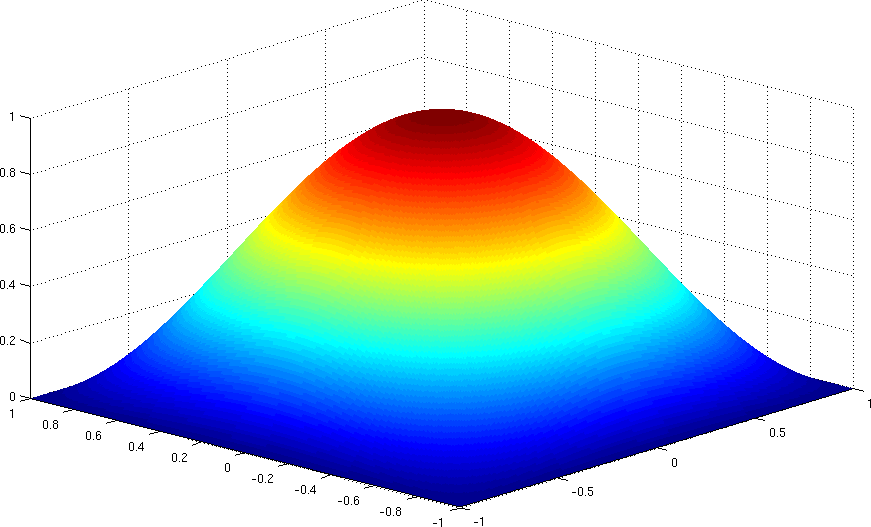
\includegraphics[width=5in,keepaspectratio=true]{./Figures/gradpField.png}
 % gradpField.png: 871x527 pixel, 90dpi, 24.59x14.88 cm, bb=0 0 697 422
 \caption{Initial pressure field}
 \label{fig:gradpField}
\end{figure}

This pressure field was chosen because $p$ is zero on all boundaries (thus eliminating the surface integral in the finite element formulation), and there is a simple analytical expression for the exact accelerations, 
$a=\left[ \begin{array}{c}
           \frac{\pi}{2}\sin(\frac{\pi}{2}x)\cos(\frac{\pi}{2}y)  \\
	    \frac{\pi}{2}\cos(\frac{\pi}{2}x)\sin(\frac{\pi}{2}y)
          \end{array}
 \right]$.

\begin{figure}[h!]
\begin{center}
$\begin{array}{c@{\hspace{.1in}}c@{\hspace{.1in}}c}
\includegraphics*[width=1.8in,keepaspectratio=true]{./Figures/gradpmesh1.png}  &  
\includegraphics*[width=1.8in,keepaspectratio=true]{./Figures/gradpmesh2.png}  &
\includegraphics*[width=1.8in,keepaspectratio=true]{./Figures/gradpmesh3.png}   \\
\end{array}$
\end{center}
\caption{Series of refined distorted meshes}
\label{fig:randomRefined}
\end{figure}

\subsection{The $\mathrm{div}(\mathrm{grad}(V))$ Test}
The $\mathrm{div}(\mathrm{grad}(V))$ test was devised to measure the accuracy and convergence rates of the several methods in approximating the $\mathrm{div}(\mathrm{grad}())$ operator, a calculation that is imperative for the tensor artificial viscosity term in shock problems. In this problem, we project a velocity field,
\[
 \begin{array}{c}
   V_x = \cos(\pi x) \cos(3 \pi y) \\
   V_y = \cos(3 \pi x) \cos(\pi y)
 \end{array}
\]
onto the mesh, $x,y \in [0,1]$. This velocity field is looks like \refFig{divgradV}. We use the same sequence of Cartesian and distorted meshes to establish convergence rates. The first measure of a method is that projection of the velocity field onto the velocity basis functions converges to the exact field under refinement. Finally, we check that the predicted accelerations due to the artificial viscosity converge to the analytically predicted value, \refEq{gradPExactA}.
\newEq{gradPExactA}{
  \begin{array}{c}
   a_x = -\pi^2 \cos(\pi x) \cos(3\pi y)+9\pi^2 \cos(\pi x) \cos(3\pi y) \\
   a_y = -9\pi^2 \cos(3\pi x) \cos(\pi y)+\pi^2 \cos(3\pi x) \cos(\pi y) \\
 \end{array} 
}
This velocity field was chosen for simplicity's sake in order to eliminate the boundary terms in the weak form description. These boundary terms vanish to zero if $\Grad V \cdot \vec{n} = 0$, where $\vec{n}$ is the outward facing unit normal vector of the domain. A simple analysis will confirm that this vector field does indeed satisfy this requirement for this particular domain. We also chose this vector field because it is complicated enough to run our method through the ringer. We have regions of converging, diverging, and swirling flow. Our stiffness matrix needs to be able to capture the details of some complicated flow fields.

\begin{figure}[h!]
 \centering
 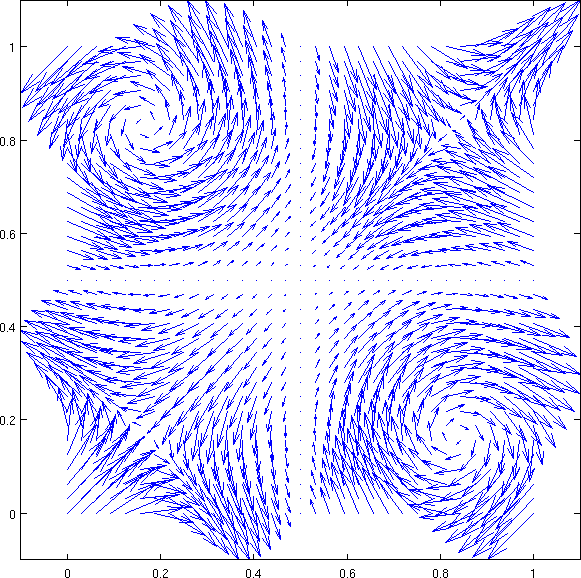
\includegraphics[width=5in]{./Figures/divgradV3.png}
 % gradpField.png: 871x527 pixel, 90dpi, 24.59x14.88 cm, bb=0 0 697 422
 \caption{Projected velocity vector field}
 \label{fig:divgradV}
\end{figure}

\section{The Acoustic Wave Test}
We discovered that a delta function disturbance is the surest way of exciting hourglass modes. In light of this, Robert Rieben developed the acoustic wave test problem to reveal whether a mixed finite element pair exhibits tendencies for hourglass mode instabilities. In this test, a single node in an initially Cartesian mesh is oscillated in time with a small amplitude. Because this is supposed to be a smooth problem and no shocks should show up, all artificial viscosity is turned off. Ideally, in an hourglass-free formulation, a simple acoustic wave will propagate through the mesh.

While useful for qualitative analysis, this test problem has several problems that exclude it from a more quantitative analysis. While it may be possible to derive an exact solution to this problem, none has been derived to our knowledge. But this is not the primary concern with this test problem. In fact, there would not be very much benefit in deriving an exact solution because it is impossible to achieve a converging solution under refinement. This is because of an inherent contradiction in the problem definition. In order to produce comparable results between methods and different mesh refinements the acoustic wave should introduce the same amount of energy to the problem. Suppose that we want to introduce a total amount of kinetic energy, $KE=\int_t \frac{1}{2}mv^2$. Therefore, in order to achieve a proportionate energy, the driving velocity must be proportional to $amp_v \propto \sqrt{\frac{KE}{m_{driver}}}$, where $amp_v$ is the amplitude of the driving velocity function and $m_{driver}$ is the mass of the driver node. Now, under refinement, $\lim_{N_z \rightarrow \infty} m_{driver} = 0$, therefore $\lim_{N_z \rightarrow \infty} amp_v = \infty$. So under refinement, as each zone shrinks in size, the driving amplitude will grow in magnitude, and adjacent cells will be crushed.

For our purposes, a $32 \times 32$ mesh provides enough resolution to accurately capture the physics while clearly illustrating hourglass modes and being coarse enough to avoid the trouble mentioned above. Ideally, we should just see the acoustic wave without any hourglass / checkerboard modes showing up. While not perfect, the \el{Q_1}{Q_0} element with a traditional hourglass filter, \refFig{acousticwave}, gives us a good idea of what we are looking for.

\begin{figure}[h!]
 \centering
 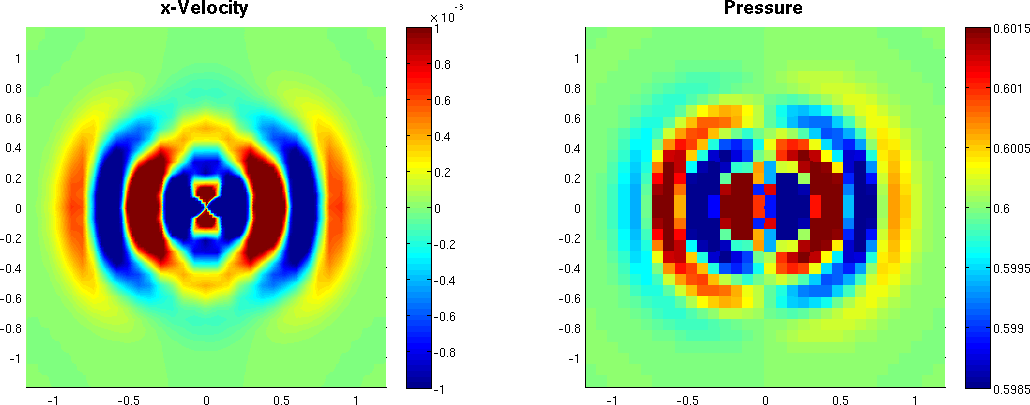
\includegraphics[width=6in,keepaspectratio=true]{./Figures/acousticQ1Q0_hgON.png}
 % elQ1Q0.png: 509x592 pixel, 107dpi, 12.08x14.05 cm, bb=0 0 342 398
 \caption{Traditional \el{Q_1}{Q_0} acoustic wave with hourglass filter}
 \label{fig:acousticwave}
\end{figure}

\section{The \texorpdfstring{\el{Q_1}{Q_0}}{Q1-Q0} Element}
Foremost among our goals is to compare the performance of any new methods with the traditional formulation, the tried and true low order \el{Q_1}{Q_0} element pair. This element has a bi-linear kinematic interpolation and a discontinuous-between-cells constant thermodynamic interpolation. A diagram of the master \el{Q_1}{Q_0} element is shown in \refFig{elQ1Q0}.

\begin{figure}[h!]
 \centering
 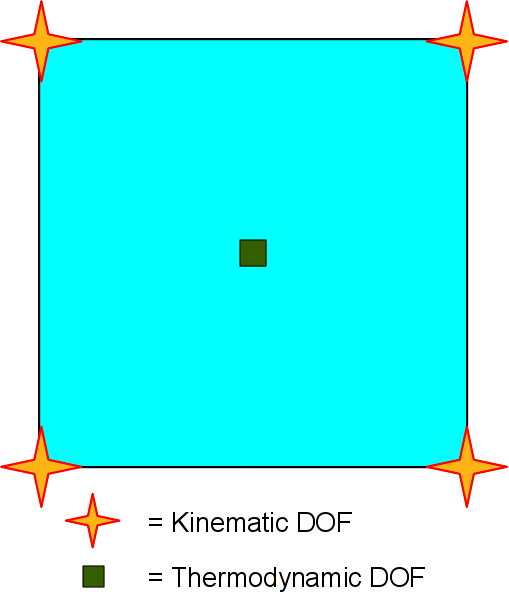
\includegraphics[width=2in,bb=0 0 342 398,keepaspectratio=true]{./Figures/elQ1Q0.png}
 % elQ1Q0.png: 509x592 pixel, 107dpi, 12.08x14.05 cm, bb=0 0 342 398
 \caption{The traditional $Q_1-\hat{Q}_0$ element}
 \label{fig:elQ1Q0}
\end{figure}

\subsection{Assets}
This element has the optimal constrain ratio of $nD$. It is simple and the legacy pair for hydrocodes, hence the theory is well developed and the problems are understood and have mostly been addressed in one form or another. 

\subsection{Liabilities}
This finite element pair has some long-standing issues because it is fundamentally unstable according to the LBB condition. Hourglass/checkerboard modes can render this method useless without an hourglass filter. Even with an hourglass filter, this method requires custom tuning for different problem types because there is no one `safe' value of the hourglass filter. This method is also low order, so it cannot accurately represent curved boundaries.

\subsection{Convergence}
We will be using this method as the `control group' with which we will compare all other methods.

\subsubsection{The $\mathrm{grad}(p)$ Test on a Cartesian Mesh}
On a straight Cartesian mesh the basis function representation of pressure converges linearly with a rate of one. This is what we would expect with piecewise constant pressures. 

The final solution converges at a super-linear rate of 1.52. This can be attributed to the well-documented super-convergence of the \el{Q_1}{Q_0} element  \cite{Douglas1985}. 

\subsubsection{The $\mathrm{grad}(p)$ Test on a Distorted Mesh}
The pressure representation converges with a rate of 1.0 on a a distorted mesh. We don't see any sort of super-convergence with the basis function representation. Thus, we don't see a significant difference between convergence on Cartesian mesh versus a distorted mesh. Henceforth we will report a single value for the convergence of the pressure representation; this will be representative for both meshes. 

With a full mass matrix solve, this method converges under refinement at a rate of 1.4, somewhat better than first order but not quite as fast as second order convergence. We will use this as the baseline to compare all other methods against. 

\subsubsection{The $\mathrm{div}(\mathrm{grad}(V))$ Test on a Cartesian Mesh}
The velocity representation of the continuous vector field converges with a rate of 2.0. This value is representative of both Cartesian and distorted meshes and we will only report one value from now on. 

The calculated accelerations converge to the analytical solution at a quadratic rate of 2.0. 

\subsubsection{The $\mathrm{div}(\mathrm{grad}(V))$ Test on a Distorted Mesh}
On a distorted mesh, the solution converges to a slightly slower rate of 1.52.

\subsection{Spurious Modes}
This finite element pair is notorious for hourglass mode instabilities. In fact, the name ``hourglass mode'' was coined because of how they manifest themselves on this element. \refFig{acousticQ1Q0_hgOFF} illustrates the excited velocity and pressure modes for this basis function pair.

\begin{figure}[h!]
 \centering
 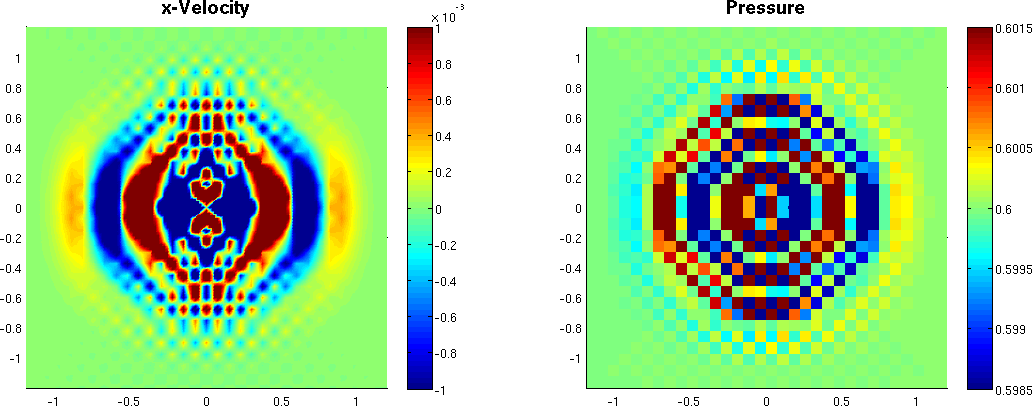
\includegraphics[width=6in,keepaspectratio=true]{./Figures/acousticQ1Q0_hgOFF.png}
 % elQ1Q0.png: 509x592 pixel, 107dpi, 12.08x14.05 cm, bb=0 0 342 398
 \caption{Traditional \el{Q_1}{Q_0} acoustic wave without hourglass filter}
 \label{fig:acousticQ1Q0_hgOFF}
\end{figure}

If we take a closer look at the spurious modes, we will see that they take the familiar hourglass/checkerboard form as illustrated on a patch of four elements in \refFig{hgmodesQ1Q0}.

\begin{figure}[h!]
 \centering
 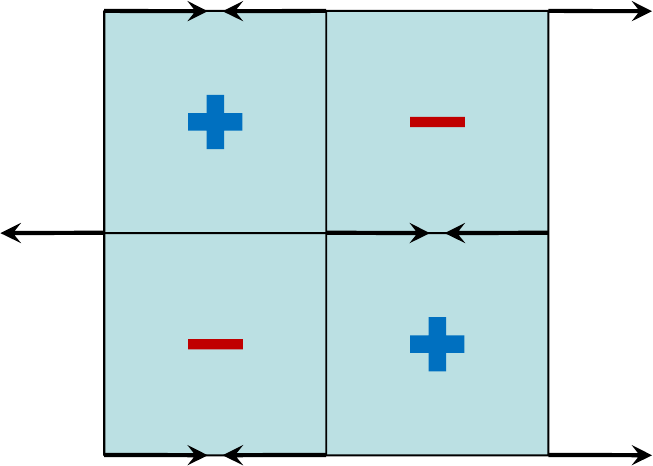
\includegraphics[width=3in,keepaspectratio=true]{./Figures/hgmodesQ1Q0.png}
 % elQ1Q0.png: 509x592 pixel, 107dpi, 12.08x14.05 cm, bb=0 0 342 398
 \caption{Hourglass/checkerboard modes on a patch of \el{Q_1}{Q_0} elements}
 \label{fig:hgmodesQ1Q0}
\end{figure} 

\section{The \texorpdfstring{\el{Q_1}{P_{0r}}}{Q1-P0r} Element}
We include this element in the discussion for the sake of thoroughness, although this element has little potential for a full hydrocode. If we wish to add one more thermodynamic degree of freedom to the \el{Q_1}{Q_0} element, we will get \refFig{elQ1P0r}. There are actually several ways that we could have distributed the two pressure DOFs, none of them great. We could have divided the element in half from top to bottom or left to right, but either of these would have doubled the amount of information in one direction versus the other. We have decided to alternatively split the element down one diagonal then the other. This acts to limit the asymmetry of the mesh.

\begin{figure}[h!]
 \centering
 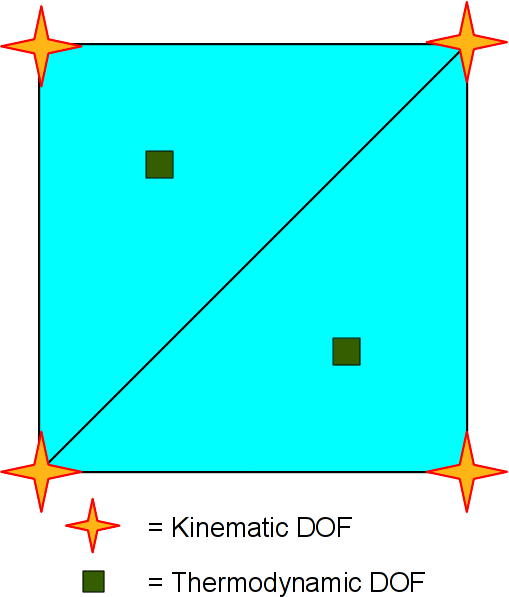
\includegraphics[width=2in,bb=0 0 342 398,keepaspectratio=true]{./Figures/elQ1P0r.png}
 % elQ1Q0.png: 509x592 pixel, 107dpi, 12.08x14.05 cm, bb=0 0 342 398
 \caption{The \el{Q_1}{\hat P_{0r}} element}
 \label{fig:elQ1P0r}
\end{figure}

\subsection{Assets}
This element may initially appear to be a straightforward extension of the traditional \el{Q_1}{Q_0} element. There are no foreseeable  advantages of using this element over any other element. In fact, there are many reasons not to use this element.

\subsection{Liabilities}
In order to limit the inherent asymmetry of this element, it is necessary to alternative placement of the two alternative versions of this element across the mesh. This means changing the software architecture to account for different basis functions depending on whether the element number is even or odd. 

\subsection{Convergence}
The pressure field converges to the exact $\mathrm{grad}(p)$ pressure field at a rate of 1.0, with only slightly less error than \el{Q_1}{Q_0}, as shown in \refFig{gp_cp_convQ1P0r}. The calculated acceleration converges sub-linearly at a rate of 0.54 as shown in \refFig{gp_ca_convQ1P0r}. Apparently, this extra degree of freedom actually slows down the convergence significantly. The $\mathrm{div}(\mathrm{grad}(V))$ convergence will be the same as \el{Q_1}{Q_0}.

\begin{figure}[h!]
 \centering
 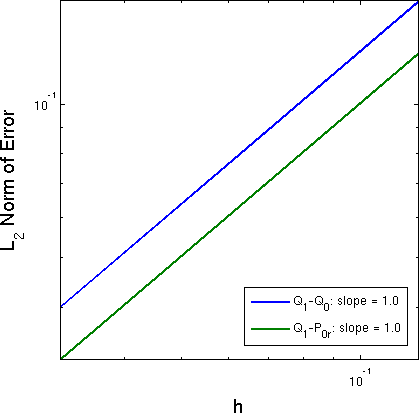
\includegraphics[width=3in,keepaspectratio=true]{./Figures/gp_cp_convQ1P0r.png}
 % elQ1Q0.png: 509x592 pixel, 107dpi, 12.08x14.05 cm, bb=0 0 342 398
 \caption{Convergence of the \el{Q_1}{P_{0r}} pressure field}
 \label{fig:gp_cp_convQ1P0r}
\end{figure}

\begin{figure}[h!]
 \centering
 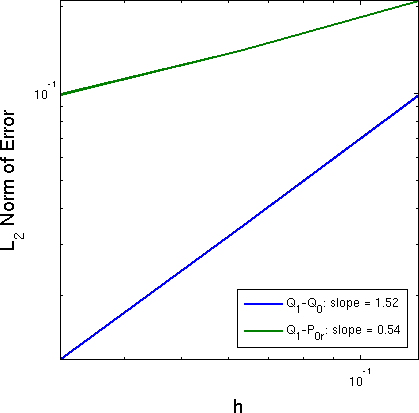
\includegraphics[width=3in,keepaspectratio=true]{./Figures/gp_ca_convQ1P0r.png}
 % elQ1Q0.png: 509x592 pixel, 107dpi, 12.08x14.05 cm, bb=0 0 342 398
 \caption{Convergence of $\Grad p$ acceleration: \el{Q_1}{P_{0r}} versus \el{Q_1}{Q_0} on a Cartesian mesh}
 \label{fig:gp_ca_convQ1P0r}
\end{figure}

\subsection{Spurious Modes}
According to \refFig{acousticQ1P0r_hgOFF}, this element does nothing to eliminate or even reduce spurious velocity and pressure modes.

\begin{figure}[h!]
 \centering
 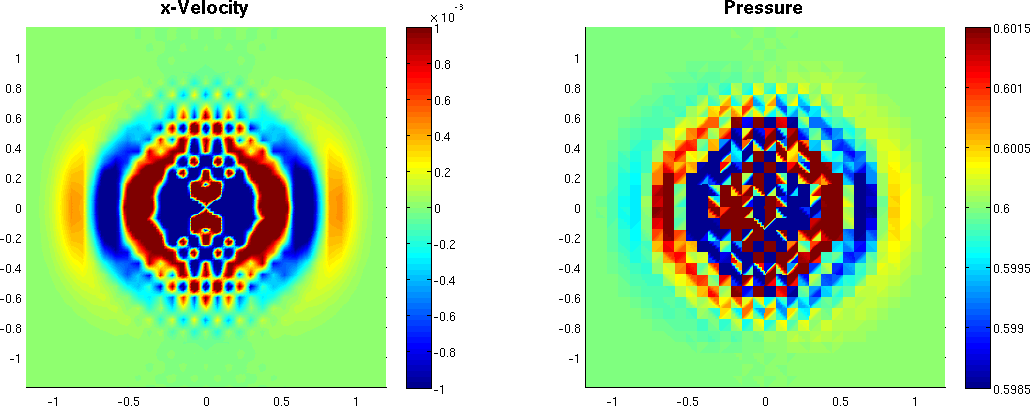
\includegraphics[width=6in,keepaspectratio=true]{./Figures/acousticQ1P0r_hgOFF.png}
 % elQ1Q0.png: 509x592 pixel, 107dpi, 12.08x14.05 cm, bb=0 0 342 398
 \caption{\el{Q_1}{P_{0r}} acoustic wave without hourglass filter}
 \label{fig:acousticQ1P0r_hgOFF}
\end{figure}

\section{The \texorpdfstring{\el{Q_1}{\hat P_1}}{Q1-P1}  Element} \label{sec:Q1P1}
We considered the \el{Q_1}{\hat P_1} and \el{Q_2}{\hat P_1} elements as a means of breaking up the hourglass modes by breaking the symmetry inherent in quad-quad pairs. 

\begin{figure}[h!]
 \centering
 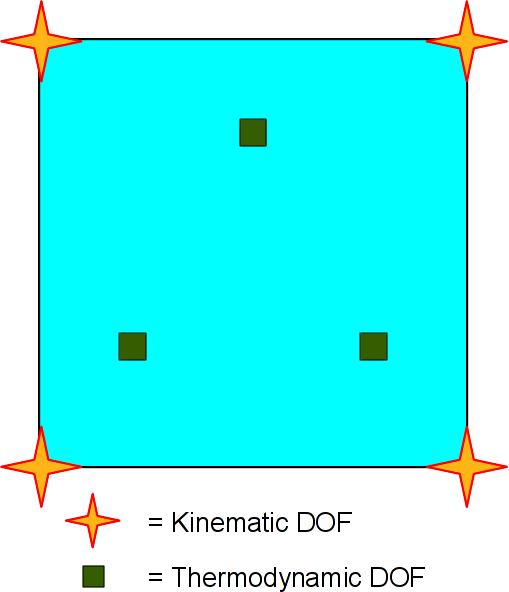
\includegraphics[width=2in,bb=0 0 342 398,keepaspectratio=true]{./Figures/elQ1P1.png}
 % elQ1Q0.png: 509x592 pixel, 107dpi, 12.08x14.05 cm, bb=0 0 342 398
 \caption{The \el{Q_1}{\hat P_1} element}
 \label{fig:elQ1P1}
\end{figure}

After some initial research, it appears that this element behaves identically to the \el{Q_1}{\hat Q_1} element. This actually more of a reflection on \el{Q_1}{\hat Q_1}; it reveals that four pressure degrees of freedom are one too many to be paired with $Q_1$ velocity basis functions. However, because \el{Q_1}{\hat Q_1} has gained so much recognition because of the method of sub-zonal pressures, we will direct our analysis at that element and limit our discussion of \el{Q_1}{\hat P_1} to this: all of the assets, liabilities, and convergence properties of \el{Q_1}{\hat P_1} will be very similar or identical to \el{Q_1}{\hat Q_1}.

\section{The \texorpdfstring{\el{Q_1}{\hat Q_1}}{Q1-Q1} Element}
This element pair, which is illustrated in \refFig{elQ1Q1}, is similar in nature to the method of sub-zonal pressures described by Caramana and Shashkov \cite{CaramanaShashkov98}. The kinematic interpolation is the same as the traditional \el{Q_1}{\hat Q_0} element, but four thermodynamic degrees of freedom are used rather than one. The method of sub-zonal pressures, on the other hand, evolved one pressure degree of freedom and calculated ``sub-zonal pressures'' each time step.

\begin{figure}[h!]
 \centering
 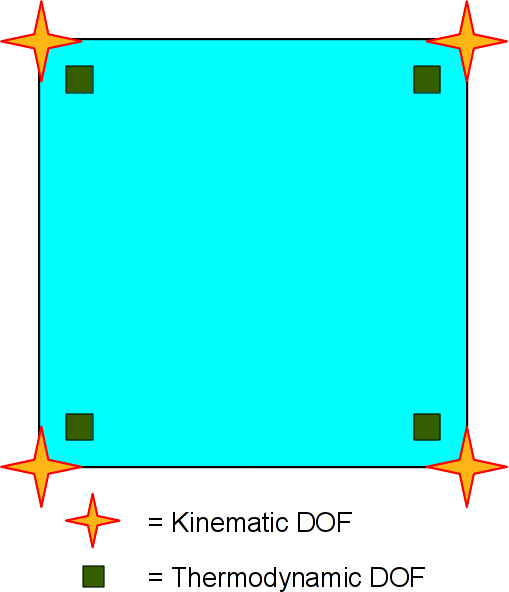
\includegraphics[width=2in,bb=0 0 342 398,keepaspectratio=true]{./Figures/elQ1Q1.png}
 % elQ1Q0.png: 509x592 pixel, 107dpi, 12.08x14.05 cm, bb=0 0 342 398
 \caption{The \el{Q_1}{\hat Q_1} element}
 \label{fig:elQ1Q1}
\end{figure}

\subsection{Assets}
On the surface, this method appears to eliminate checkerboard modes from the pressure field. This seems like it could be an attractively easy fix for checkerboard mode instabilities that does not require special tuning between problems. \refFig{centerPresQ1Q1} shows the resulting average pressures in each cell for the acoustic wave problem.

\begin{figure}[h!]
 \centering
 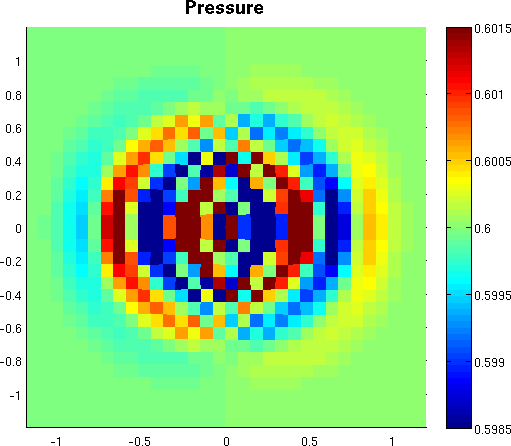
\includegraphics[width=5in,keepaspectratio=true]{./Figures/centerPresQ1Q1.png}
 % elQ1Q0.png: 509x592 pixel, 107dpi, 12.08x14.05 cm, bb=0 0 342 398
 \caption{Average pressure in each cell for \el{Q_1}{\hat Q_1} element for acoustic wave problem}
 \label{fig:centerPresQ1Q1}
\end{figure}

\subsection{Liabilities}
The constraint ratio for this element is $nD/4$, but let's not let that discourage us. We haven't proven whether this is a viable measure of performance yet. We have also shown previously in \refSec{Q1P1} that this element has one too many thermodynamic degrees of freedom. The major downfall of this element comes when we take a closer look at the resulting velocity field. Apparently, \refFig{centerPresQ1Q1} just hid the spurious pressure modes by averaging the pressure degrees of freedom because \refFig{spuriousVQ1Q1} shows that spurious velocity modes in the x- and y- directions. This plot should look more like \refFig{spuriousVQ1Q0}. These spurious modes appear to be more chaotic than \el{Q_1}{Q_0} and may be harder to control.

\begin{figure}[h!]
 \centering
 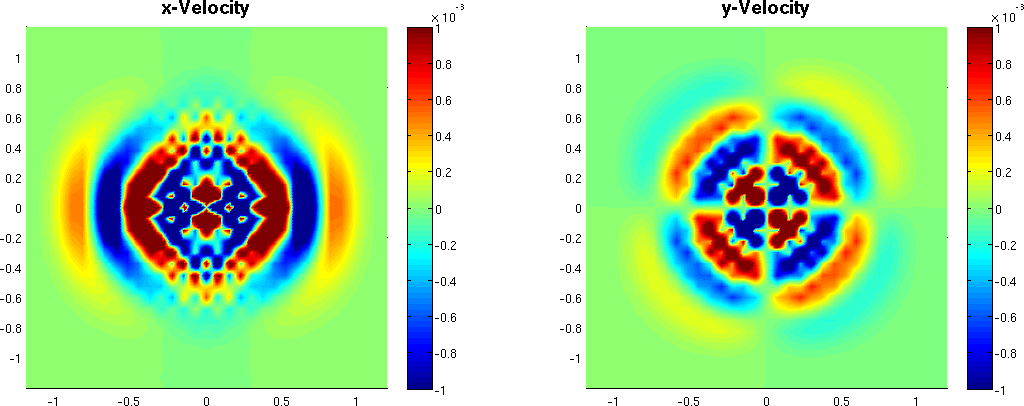
\includegraphics[width=6in,keepaspectratio=true]{./Figures/acousticSpuriousV_Q1Q1.png}
 \caption{Spurious modes in the x- and y-velocity modes with \el{Q_1}{\hat Q_1}}
 \label{fig:spuriousVQ1Q1}
\end{figure}

\begin{figure}[h!]
 \centering
 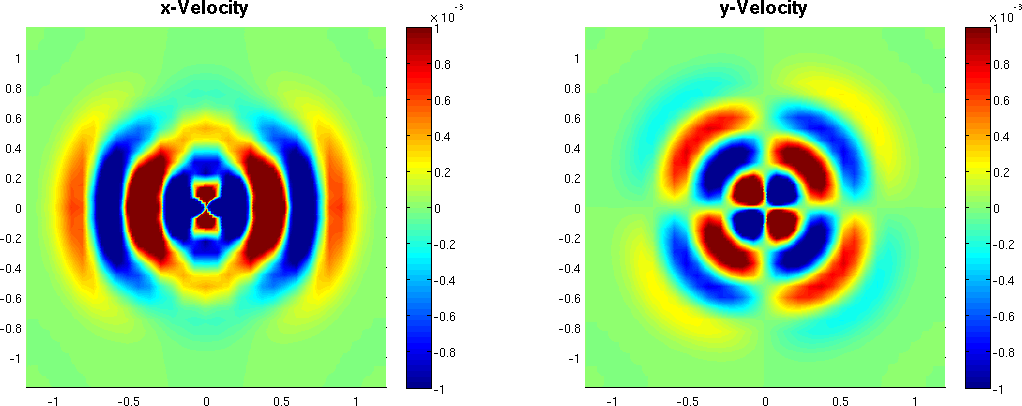
\includegraphics[width=6in,keepaspectratio=true]{./Figures/acousticSpuriousV_Q1Q0.png}
 \caption{Hourglass-free velocity fields with hourglass-filtered \el{Q_1}{Q_0}}
 \label{fig:spuriousVQ1Q0}
\end{figure}

\subsection{Convergence}

\subsubsection{The $\mathrm{grad}(p)$ Test on a Cartesian Mesh}
The pressure representation converges to the continuous pressure field at a quadratic rate of 2.0. This element shares the same pressure representation as the \el{Q_2}{\hat Q_1} element, therefore the pressure field convergence is the same. See \refFig{gp_cp_convQ2Q1} for the convergence of the pressure field of these two elements.

On a Cartesian mesh, the static momentum test converges with a rate of 2.0 as shown in \refFig{gp_ca_convQ1Q1}.

\begin{figure}[h!]
 \centering
 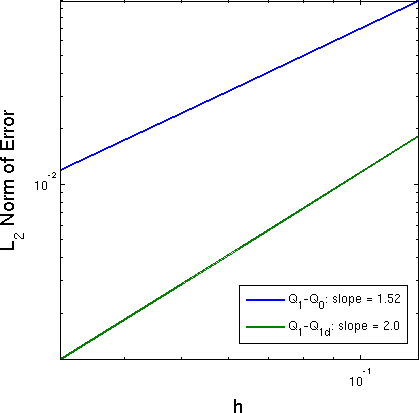
\includegraphics[width=3in,keepaspectratio=true]{./Figures/gp_ca_convQ1Q1.png}
 % elQ1Q0.png: 509x592 pixel, 107dpi, 12.08x14.05 cm, bb=0 0 342 398
 \caption{Convergence of $\Grad p$ acceleration: \el{Q_1}{\hat Q_1} versus \el{Q_1}{Q_0} on a Cartesian mesh}
 \label{fig:gp_ca_convQ1Q1}
\end{figure}

\subsubsection{The $\mathrm{grad}(p)$ Test on a Distorted Mesh}
Despite its deficiencies, this method does converge to the exact solution on a distorted mesh with quadratic convergence as shown in \refFig{gp_da_convQ1Q1}.

\begin{figure}[h!]
 \centering
 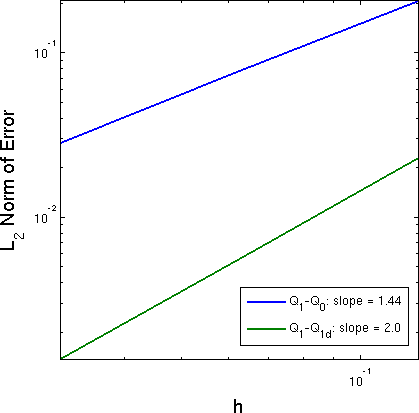
\includegraphics[width=3in,keepaspectratio=true]{./Figures/gp_da_convQ1Q1.png}
 % elQ1Q0.png: 509x592 pixel, 107dpi, 12.08x14.05 cm, bb=0 0 342 398
 \caption{Convergence of $\Grad p$ acceleration: \el{Q_1}{\hat Q_1} versus \el{Q_1}{Q_0} on a distorted mesh}
 \label{fig:gp_da_convQ1Q1}
\end{figure}

\subsubsection{The $\mathrm{div}(\mathrm{grad}(V))$ Test}
It turns out that the stiffness matrix depends entirely on the velocity space. Therefore, the \el{Q_1}{\hat Q_1} element behaves identically to the \el{Q_1}{Q_0} element for $\mathrm{div}(\mathrm{grad}(V))$ test. The pressure space has nothing to do with the results. 

\subsection{Spurious Modes}\label{sec:Q1Q1spuriousmodes}
If we actually plot the bi-linear interpolation of pressure rather than the average value, we will see that the pressure field is not as pretty as we thought. \refFig{acousticQ1Q1_hgOFF} shows the pseudocolor plot for this element on the acoustic wave test.

\begin{figure}[h!]
 \centering
 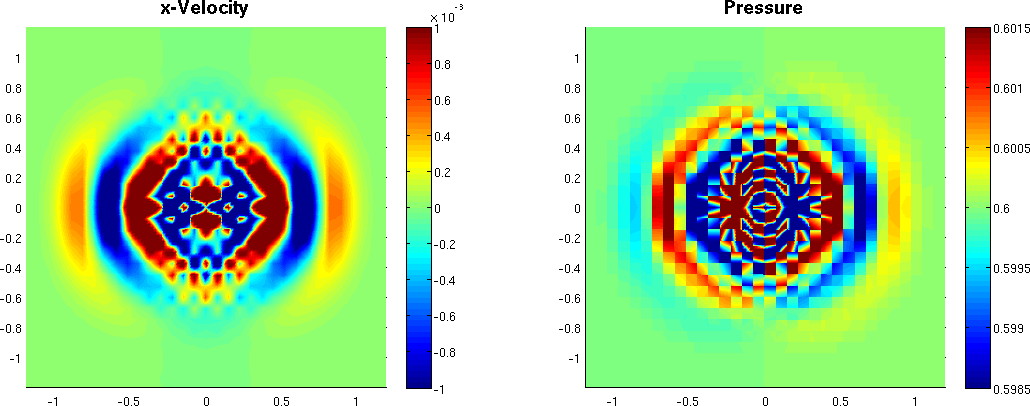
\includegraphics[width=6in,keepaspectratio=true]{./Figures/acousticQ1Q1_hgOFF.png}
 % elQ1Q0.png: 509x592 pixel, 107dpi, 12.08x14.05 cm, bb=0 0 342 398
 \caption{\el{Q_1}{\hat Q_1} acoustic wave without hourglass filter}
 \label{fig:acousticQ1Q1_hgOFF}
\end{figure}

\section{The \texorpdfstring{\el{Q_1}{\hat Q_2}}{Q1-Q2} Element}
In order to be completely thorough, we briefly explored further enriching the pressure space, see \refFig{elQ1Q2}. It turns out that there are not enough velocity DOFs to produce a full bi-quadratic pressure field, but unlike the \el{Q_2}{Q_0} element which has the reverse problem, this is not a fatal flaw. The extra thermodynamic DOFs end up just taking on a bi-linear shape and thus are superfluous. The same problems plague this element as \el{Q_1}{\hat Q_1}.

\begin{figure}[h!]
 \centering
 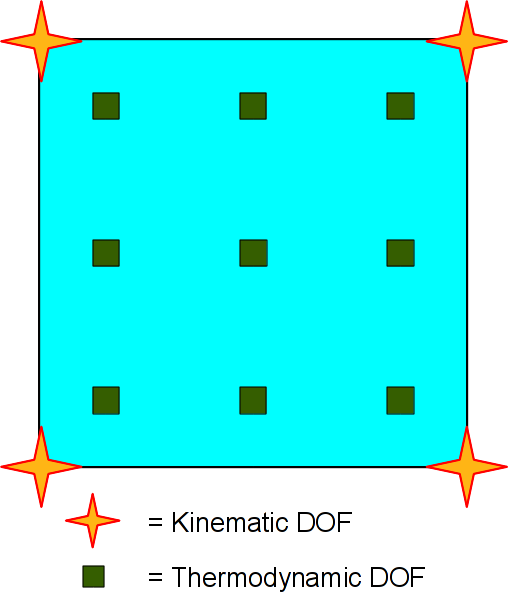
\includegraphics[width=2in,bb=0 0 342 398,keepaspectratio=true]{./Figures/elQ1Q2.png}
 % elQ1Q0.png: 509x592 pixel, 107dpi, 12.08x14.05 cm, bb=0 0 342 398
 \caption{The \el{Q_1}{\hat Q_2} element}
 \label{fig:elQ1Q2}
\end{figure}

\section{The \texorpdfstring{\el{Q_2}{Q_0}}{Q2-Q0} Element}
One of our early attempts to correct hourglass mode instabilities was to follow the lead of some research in Stokes flow and enrich the velocity space. This led to the \el{Q_2}{Q_0} element and caused us to reconsider the applicability of Stokes flow elements to inviscid flow. 

\begin{figure}[h!]
 \centering
 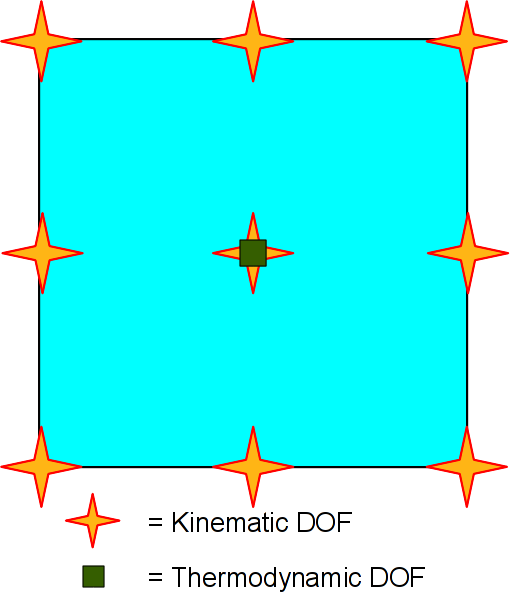
\includegraphics[width=2in,bb=0 0 342 398,keepaspectratio=true]{./Figures/elQ2Q0.png}
 % elQ1Q0.png: 509x592 pixel, 107dpi, 12.08x14.05 cm, bb=0 0 342 398
 \caption{The \el{Q_2}{Q_0} element}
 \label{fig:elQ2Q0}
\end{figure}

\subsection{Assets}
Analysis of the inf-sup condition by Stenberg and Suri \cite{StenbergSuri1996} showed that \el{Q_{k+2}}{Q_k} family of elements is stable for Stokes flow. The \el{Q_2}{Q_0} element falls into this family, but it is not stable for Euler flow.

\subsection{Liabilities}
It turns out that, while this element may work for Stokes flow, there are not enough pressure degrees of freedom to inform the movement of all of the higher order velocity degrees of freedom. The internal degree of freedom, for example, does not ever see any pressure gradient because pressure is constant within each cell. Therefore, the central DOF never moves.

\subsection{Convergence}
This finite element pair does not converge at all, which renders it completely unsuitable for a hydrocode.

\section{The \texorpdfstring{\el{Q_2}{\hat P_1}}{Q2-P1} Element}
One element that showed some unexpected promise was the \el{Q_2}{\hat P_1} element. This element has a bi-quadratic kinematic interpolation and a linear thermodynamic interpolation as depicted in \refFig{elQ2P1}.

\begin{figure}[h!]
 \centering
 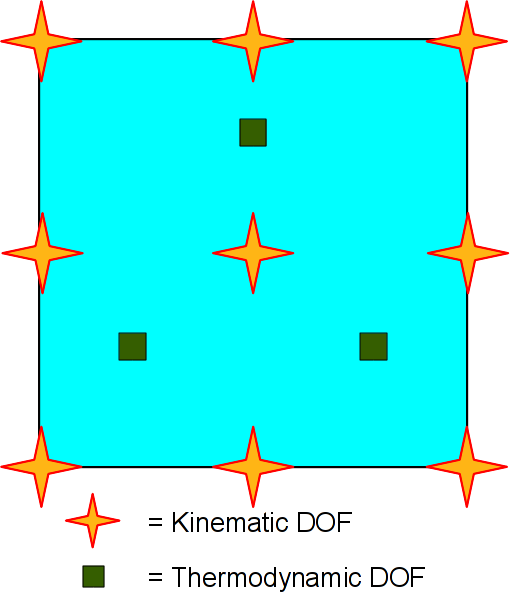
\includegraphics[width=2in,bb=0 0 342 398,keepaspectratio=true]{./Figures/elQ2P1.png}
 % elQ1Q0.png: 509x592 pixel, 107dpi, 12.08x14.05 cm, bb=0 0 342 398
 \caption{The \el{Q_2}{\hat P_1} element}
 \label{fig:elQ2P1}
\end{figure}

\subsection{Assets}
With its bi-quadratic spatial interpolation, this element is capable of producing curved geometries. Similar to the other $Q_2$ elements, this allows us to calculate second derivatives within a single cell while better representing higher-order phenomena with fewer zones and faster convergence. Three pressure DOFs is also the fewest degrees of freedom needed to fully inform the movement of all 9 higher-order velocity degrees of freedom. This means that we can calculate thermodynamic gradients with ease.

\subsection{Liabilities}
Probably the principle oddity of this element lies in the fact that we have ``embedded'' a 3-point basis function on a quadrilateral. There is no real reason why this shouldn't be done, at least for the thermodynamic space, but there is an element of uncertainty about this. If we are using quads, shouldn't we use quad-based basis functions? Where are the most natural locations for these three DOFs? Despite it's higher order nature, this element appears to have slower convergence characteristics on the $\mathrm{grad}(p)$ test than traditional methods. Thus it seems that \el{Q_2}{\hat Q_1} is the preferred higher order method.
% One consequence that could hurt the efficiency of this method is that the thermodynamic DOFs may not line up perfectly with the quadrature points used as 

\subsection{Convergence}
This element has disappointing convergence trends. 

\subsubsection{The $\mathrm{grad}(p)$ Test}
The pressure field representation is the same as for \el{Q_1}{\hat P_1}. The solution converges at a rate of 1.25 which is actually sub-standard compared to \el{Q_1}{Q_0}.

\begin{figure}[h!]
 \centering
 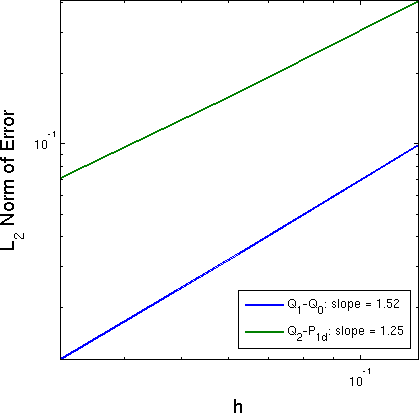
\includegraphics[width=3in,keepaspectratio=true]{./Figures/gp_ca_convQ2P1.png}
 % elQ1Q0.png: 509x592 pixel, 107dpi, 12.08x14.05 cm, bb=0 0 342 398
 \caption{Convergence of $\Grad p$ acceleration: \el{Q_2}{\hat P_1} versus \el{Q_1}{Q_0} on a Cartesian mesh}
 \label{fig:gp_ca_convQ2P1}
\end{figure}

When we distort the mesh, we get an even lower convergence rate of 1.20.

\begin{figure}[h!]
 \centering
 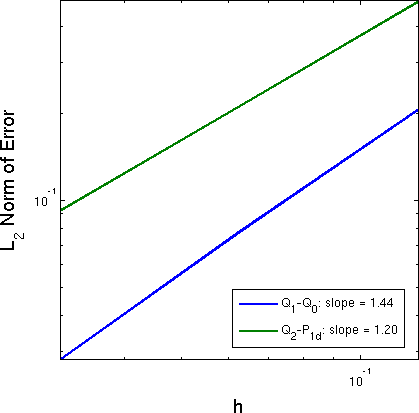
\includegraphics[width=3in,keepaspectratio=true]{./Figures/gp_da_convQ2P1.png}
 % elQ1Q0.png: 509x592 pixel, 107dpi, 12.08x14.05 cm, bb=0 0 342 398
 \caption{Convergence of $\Grad p$ acceleration: \el{Q_2}{\hat P_1} versus \el{Q_1}{Q_0} on a distorted mesh}
 \label{fig:gp_da_convQ2P1}
\end{figure}

\subsubsection{The $\mathrm{div}(\mathrm{grad}(V))$ Test}
Please see \refSec{convdgQ2Q1} for the convergence on the $\mathrm{div}(\mathrm{grad}(V))$ test.

\subsection{Spurious Modes}
The principle benefit of this element over its \el{Q_2}{\hat Q_1} cousin is that the spurious modes appear to be much more low key, see \refFig{acousticQ2Q1_hgOFF} and especially \refFig{acousticQ2Q1_hgON}.

\begin{figure}[h!]
 \centering
 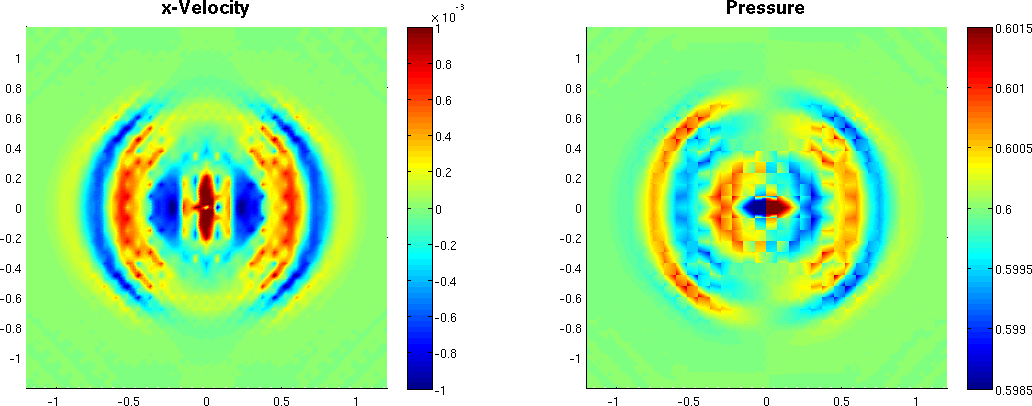
\includegraphics[width=6in,keepaspectratio=true]{./Figures/acousticQ2P1_hgOFF.png}
 % elQ1Q0.png: 509x592 pixel, 107dpi, 12.08x14.05 cm, bb=0 0 342 398
 \caption{\el{Q_2}{\hat P_1} acoustic wave without hourglass filter}
 \label{fig:acousticQ2P1_hgOFF}
\end{figure}

\begin{figure}[h!]
 \centering
 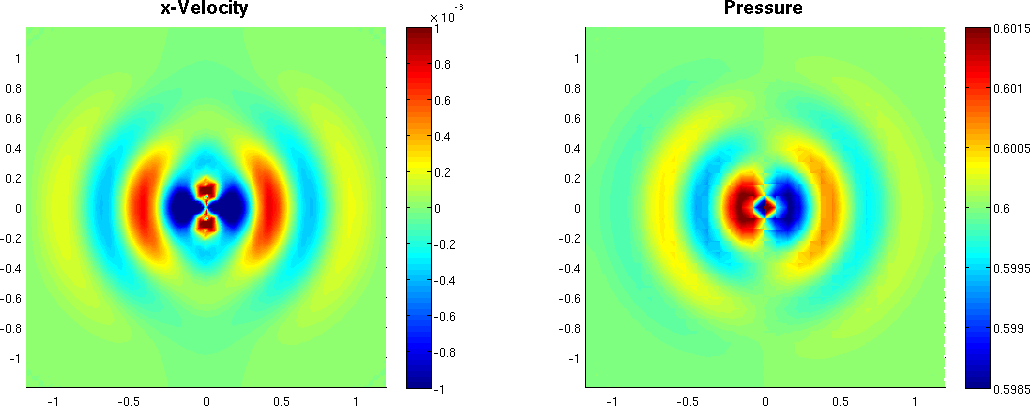
\includegraphics[width=6in,keepaspectratio=true]{./Figures/acousticQ2P1_hgON.png}
 % elQ1Q0.png: 509x592 pixel, 107dpi, 12.08x14.05 cm, bb=0 0 342 398
 \caption{\el{Q_2}{\hat P_1} acoustic wave with hourglass filter}
 \label{fig:acousticQ2P1_hgON}
\end{figure}

\section{The \texorpdfstring{\el{Q_2}{\hat Q_1}}{Q2-Q1} Element}
The logical high-order extension of classical staggered grid hydrodynamics is the \el{Q_2}{\hat Q_1} mixed finite element pair. If we enrich both the kinematic and thermodynamic basis functions by one order, we arrive at a bi-quadratic interpolation for velocity and position and a bi-linear interpolation for pressure, density, and energy, as illustrated in \refFig{elQ2Q1}. This higher order representation of the kinematic variables allows for curvilinear edges and makes it possible to calculate second derivatives within each cell. The bi-linear representation of thermodynamic variables allows us to calculate pressure, energy, and density gradient within each cell. This property could make some sub-zonal physics / multi-material capabilities more straightforward to implement in a full-scale multi-physics hydrocode.

\begin{figure}[h!]
 \centering
 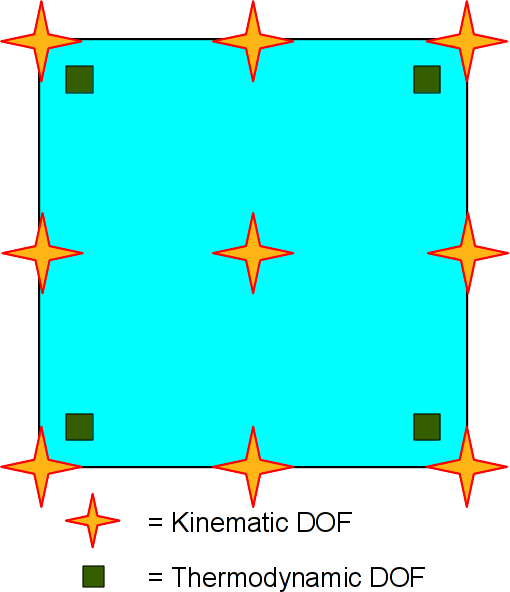
\includegraphics[width=2in,bb=0 0 342 398,keepaspectratio=true]{./Figures/elQ2Q1.png}
 % elQ1Q0.png: 509x592 pixel, 107dpi, 12.08x14.05 cm, bb=0 0 342 398
 \caption{The \el{Q_2}{\hat Q_1} element}
 \label{fig:elQ2Q1}
\end{figure}

\subsection{Assets}
This basis function pair has the optimal constraint ratio of $nD$. This is not a radical departure from traditional SGH; we are only raising the order of each interpolation by one. Therefore this is analogous to a higher order version of traditional SGH, and some of the accumulated knowledge of SGH may carry over to this method. Higher order representations of the variables allow for more accurate calculations and faster convergence while allowing us to model more complicated physics with fewer elements. We will further explore the benefits of this element in \refChap{NumericalResults}

\subsection{Liabilities}
Because this element is analogous to traditional SGH, it shares some of the same pitfalls. For example, hourglass modes take on a very similar, higher order form with \el{Q_2}{\hat Q_1}. Another possible downside to this element is that there are more possible situations where a zero or negative Jacobian could kill a simulation. For example, if the internal DOF moves more than 25\% of the cell length in any direction, the Jacobian will go negative in part of the cell. In practice, for the test problems considered, this has not been a problem, but more study is required. Also, because this is a new method, new analysis must be conducted as to stable time steps, flux between cells during the mesh relaxation stage, etc. We expect a fuller understanding of the pros and cons of this element to come out with time and further study. 

\subsection{Convergence}
This element has an attractive set of convergence properties.

\subsubsection{The $\mathrm{grad}(p)$ Test on a Cartesian Mesh}
The basis function representation of the continuous pressure field converges quadratically with a rate of 2.0 as shown in \refFig{gp_cp_convQ2Q1}.

\begin{figure}[h!]
 \centering
 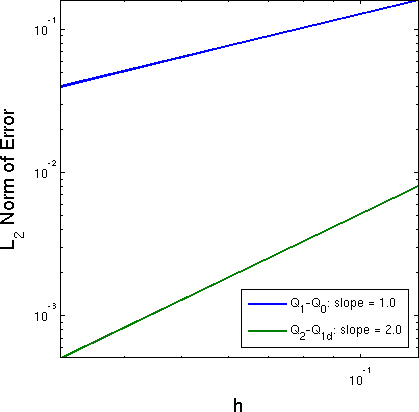
\includegraphics[width=3in,keepaspectratio=true]{./Figures/gp_cp_convQ2Q1.png}
 % elQ1Q0.png: 509x592 pixel, 107dpi, 12.08x14.05 cm, bb=0 0 342 398
 \caption{Convergence of the \el{Q_2}{\hat Q_1} pressure field}
 \label{fig:gp_cp_convQ2Q1}
\end{figure}

On a Cartesian mesh, this element converges quadratically to the analytical solution of the $\mathrm{grad}(p)$ test as shown in \refFig{gp_ca_convQ2Q1}. This is only slightly better than the \el{Q_1}{Q_0} rate of 1.52, but \refFig{gp_ca_convQ2Q1} demonstrates that the actual absolute value of error is much lower.

\begin{figure}[h!]
 \centering
 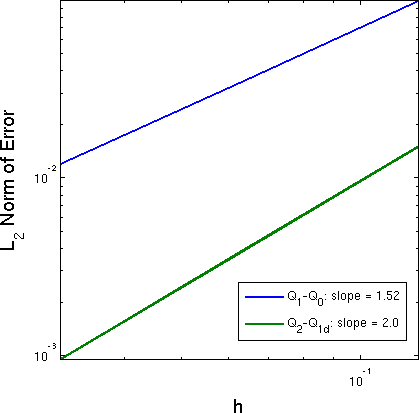
\includegraphics[width=3in,keepaspectratio=true]{./Figures/gp_ca_convQ2Q1.png}
 % elQ1Q0.png: 509x592 pixel, 107dpi, 12.08x14.05 cm, bb=0 0 342 398
 \caption{Convergence of $\Grad p$ acceleration: \el{Q_2}{\hat Q_1} versus \el{Q_1}{Q_0} on a Cartesian mesh}
 \label{fig:gp_ca_convQ2Q1}
\end{figure}

\subsubsection{The $\mathrm{grad}(p)$ Test on a Distorted Mesh}
The convergence on a distorted mesh is the real test of an element because we don't expect to see any perfectly Cartesian meshes in any simulations of real engineering interest. On the distorted mesh, the \el{Q_1}{Q_0} element drops to a rate of 1.44 while the \el{Q_2}{\hat Q_1} element drops to a slightly sub-quadratic convergence of 1.88 as shown in \refFig{gp_da_convQ2Q1}.

Interestingly, even though the \el{Q_2}{\hat Q_1} element has the same pressure space as \el{Q_1}{\hat Q_1}, it doesn't quite maintain the same rate of convergence on a distorted mesh. This difference is minor, but a little unexpected. \refFig{gp_da_convQ1Q1_Q2Q1} compares the convergence of these two elements.

\begin{figure}[h!]
 \centering
 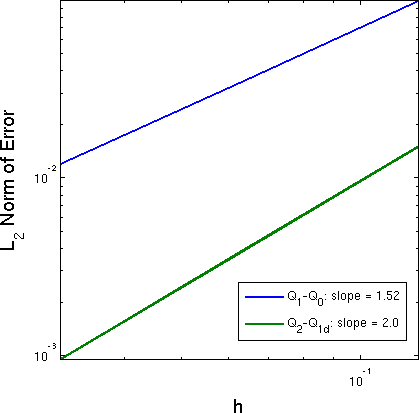
\includegraphics[width=3in,keepaspectratio=true]{./Figures/gp_ca_convQ2Q1.png}
 % elQ1Q0.png: 509x592 pixel, 107dpi, 12.08x14.05 cm, bb=0 0 342 398
 \caption{Convergence of $\Grad p$ acceleration: \el{Q_2}{\hat Q_1} versus \el{Q_1}{Q_0} on a distorted mesh}
 \label{fig:gp_da_convQ2Q1}
\end{figure}

\begin{figure}[h!]
 \centering
 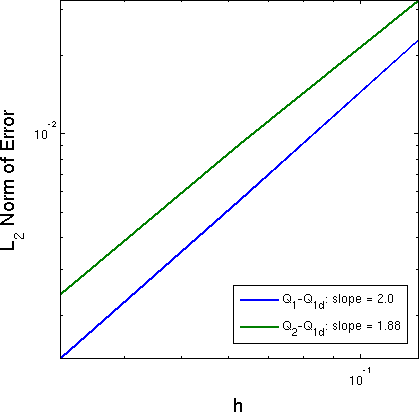
\includegraphics[width=3in,keepaspectratio=true]{./Figures/gp_da_convQ1Q1_Q2Q1.png}
 % elQ1Q0.png: 509x592 pixel, 107dpi, 12.08x14.05 cm, bb=0 0 342 398
 \caption{Convergence of $\Grad p$ acceleration: \el{Q_2}{\hat Q_1} versus \el{Q_1}{Q_1} on a distorted mesh}
 \label{fig:gp_da_convQ1Q1_Q2Q1}
\end{figure}

\subsubsection{The $\mathrm{div}(\mathrm{grad}(V))$ Test on a Cartesian Mesh}\label{sec:convdgQ2Q1}
The velocity projection converges cubically at a rate of 3.0 as shown in \refFig{dg_cV_convQ2Q1}.

\begin{figure}[h!]
 \centering
 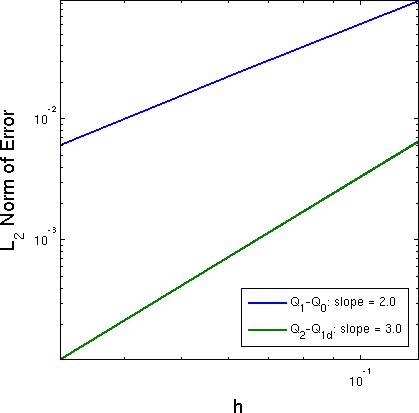
\includegraphics[width=3in,keepaspectratio=true]{./Figures/dg_cV_convQ2Q1.png}
 % elQ1Q0.png: 509x592 pixel, 107dpi, 12.08x14.05 cm, bb=0 0 342 398
 \caption{Convergence of the \el{Q_2}{\hat Q_1} velocity projection vs \el{Q_1}{Q_0}}
 \label{fig:dg_cV_convQ2Q1}
\end{figure}

The \el{Q_2}{\hat Q_1} element converges to the exact solution of the $\mathrm{div}(\mathrm{grad}(V))$ test at a rate of 2.0 on a Cartesian mesh as shown in \refFig{dg_ca_convQ2Q1}. This appears to be somewhat of an anomaly because we expect that the higher order velocity field will result in higher-order convergence.

\begin{figure}[h!]
 \centering
 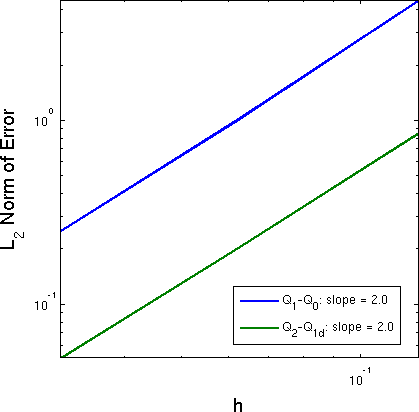
\includegraphics[width=3in,keepaspectratio=true]{./Figures/dg_ca_convQ2Q1.png}
 % elQ1Q0.png: 509x592 pixel, 107dpi, 12.08x14.05 cm, bb=0 0 342 398
 \caption{Convergence of $\Div\Grad V$ acceleration: \el{Q_2}{\hat Q_1} versus \el{Q_1}{Q_0} on a Cartesian mesh}
 \label{fig:dg_ca_convQ2Q1}
\end{figure}

\subsubsection{The $\mathrm{div}(\mathrm{grad}(V))$ Test on a Distorted Mesh}
On a distorted mesh, the convergence of both \el{Q_1}{Q_0} and \el{Q_2}{\hat Q_1} drop to sub-quadratic convergence of 1.52 and 1.63, respectively as shown in \refFig{dg_da_convQ2Q1}.

\begin{figure}[h!]
 \centering
 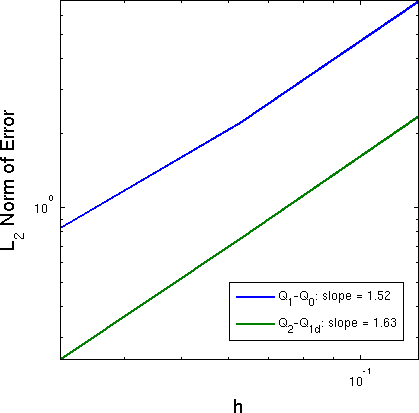
\includegraphics[width=3in,keepaspectratio=true]{./Figures/dg_da_convQ2Q1.png}
 % elQ1Q0.png: 509x592 pixel, 107dpi, 12.08x14.05 cm, bb=0 0 342 398
 \caption{Convergence of $\Div\Grad V$ acceleration: \el{Q_2}{\hat Q_1} versus \el{Q_1}{Q_0} on a distorted mesh}
 \label{fig:dg_da_convQ2Q1}
\end{figure}

\subsection{Spurious Modes}
To our disappointment, this element did not eliminate hourglass/checkerboard modes. In fact, the spurious modes present in this element bear a striking resemblance to the traditional hourglass modes found in the \el{Q_1}{Q_0} element. \refFig{acousticQ2Q1_hgOFF} shows the hourglass modes on the acoustic wave test.

\begin{figure}[h!]
 \centering
 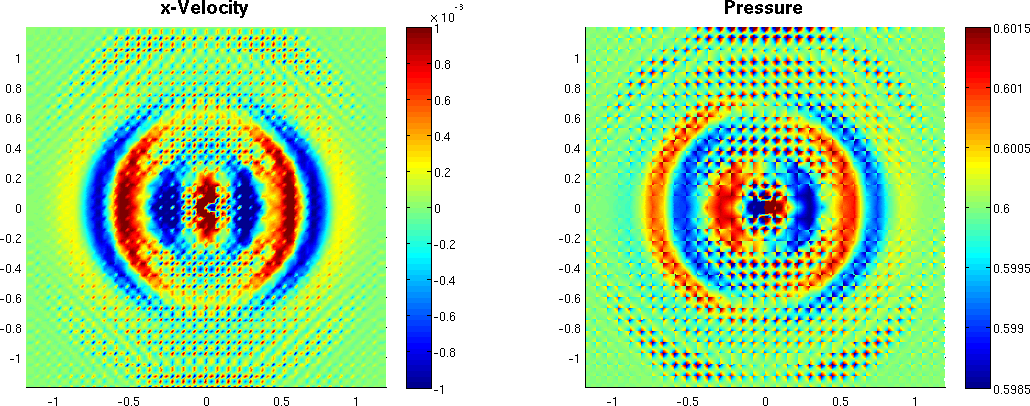
\includegraphics[width=6in,keepaspectratio=true]{./Figures/acousticQ2Q1_hgOFF.png}
 % elQ1Q0.png: 509x592 pixel, 107dpi, 12.08x14.05 cm, bb=0 0 342 398
 \caption{\el{Q_2}{\hat Q_1} acoustic wave without hourglass filter}
 \label{fig:acousticQ2Q1_hgOFF}
\end{figure}

If you look closely, you will see that these spurious modes look exactly like a higher frequency version of hourglass modes. The structure of these hourglass modes is illustrated in \refFig{hgmodesQ2Q1}. Compared to some of the other more random spurious modes that we have considered, these more structured modes work to our advantage. They should be easier to analyze and filter, especially considering their similarity to the well-studied \el{Q_1}{Q_0} hourglass modes. You may also notice in comparing \refFig{acousticQ1Q0_hgOFF} and \refFig{acousticQ2Q1_hgOFF}, that the higher frequency modes of \el{Q_2}{\hat Q_1} appear to be of lower magnitude and thus disturb the solution to a smaller degree. Despite the noise from the hourglass modes, we can see a very well defined solution. This will come in handy again as we consider the Sedov explosion test in \refChap{NumericalResults}. If we apply a filter to smooth the hourglass modes,the solution to the acoustic wave problem comes through much clearer in \refFig{acousticQ2Q1_hgON}.

\begin{figure}[h!]
 \centering
 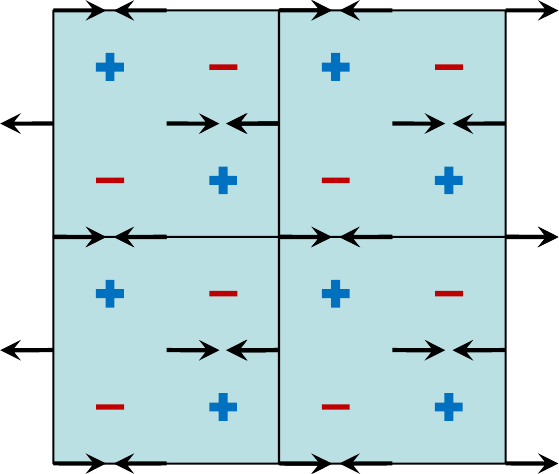
\includegraphics[width=3in,keepaspectratio=true]{./Figures/hgmodesQ2Q1.png}
 % elQ1Q0.png: 509x592 pixel, 107dpi, 12.08x14.05 cm, bb=0 0 342 398
 \caption{Hourglass/checkerboard modes on a patch of \el{Q_2}{\hat Q_1} elements}
 \label{fig:hgmodesQ2Q1}
\end{figure} 

\begin{figure}[h!]
 \centering
 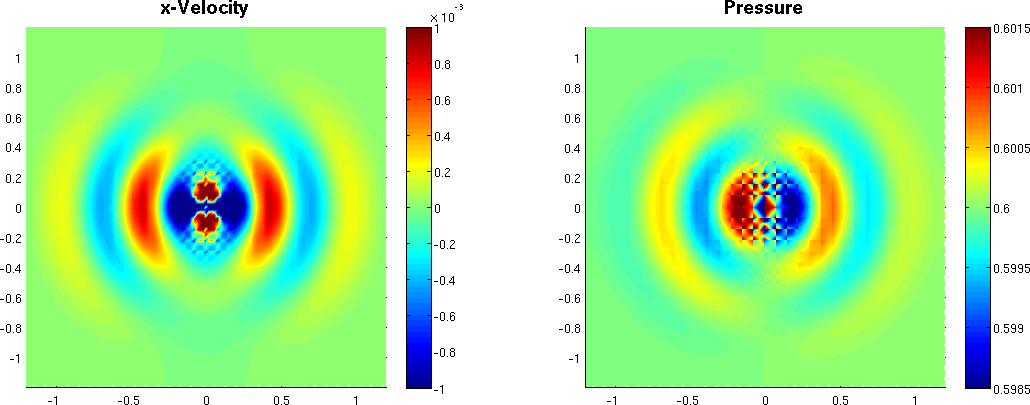
\includegraphics[width=6in,keepaspectratio=true]{./Figures/acousticQ2Q1_hgON.png}
 % elQ1Q0.png: 509x592 pixel, 107dpi, 12.08x14.05 cm, bb=0 0 342 398
 \caption{\el{Q_2}{\hat Q_1} acoustic wave with hourglass filter}
 \label{fig:acousticQ2Q1_hgON}
\end{figure}

This filtered solution looks much better even than the filtered \el{Q_1}{Q_0} solution in \refFig{acousticQ1Q0_hgOFF}.

\section{The \texorpdfstring{\el{Q_2}{\hat Q_2}}{Q2-Q2} Element}
We also tried further refining the thermodynamic space to see what it could buy us. The \el{Q_1}{\hat Q_2} element is a higher order analog of the \el{Q_1}{\hat Q_1} element with both spatial and state variables using a bi-quadratic interpolation. Similar to the \el{Q_1}{\hat Q_2} element, any higher thermodynamic representation like \el{Q_2}{\hat Q_3} appears to be redundant.

\subsection{Assets}
This element shares a lot of the same benefits and handicaps of the \el{Q_1}{\hat Q_1} element. At first glance, if you average the pressure DOFs in each zone, it appears to eliminate checkerboard modes as shown in \refFig{centerPresQ2Q2}, similar to \el{Q_1}{\hat Q_1}. But if we look at the whole picture in \refFig{acousticQ2Q2_hgOFF}, the spurious modes are actually very ugly for this element. We will see in \refSec{nohQ2Q2} that this element appears to arrest density undershoots in the Noh implosion problem. This element also shares the same spatial interpolation with \el{Q_2}{\hat Q_1} which lets this element take on curvilinear geometries. As with \el{Q_2}{\hat Q_1}, we can take second derivatives in space and compute gradients of the thermodynamic fields in a very straightforward way.

\begin{figure}[h!]
 \centering
 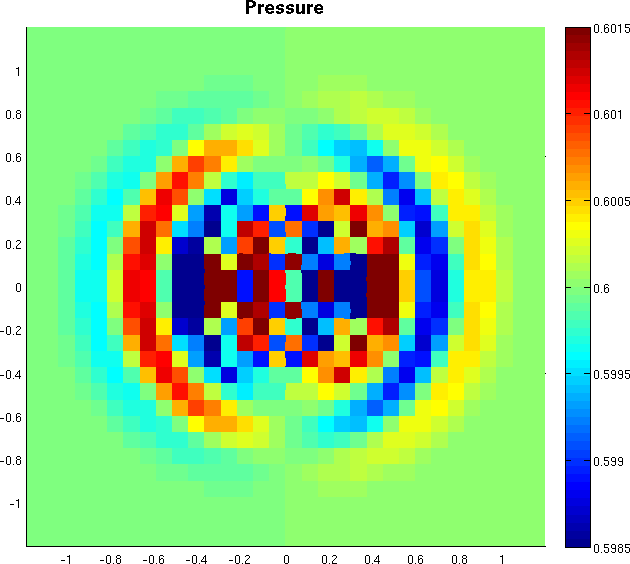
\includegraphics[width=5in,keepaspectratio=true]{./Figures/centerPresQ2Q2.png}
 % elQ1Q0.png: 509x592 pixel, 107dpi, 12.08x14.05 cm, bb=0 0 342 398
 \caption{Average pressure in each cell for \el{Q_2}{\hat Q_2} element for acoustic wave problem}
 \label{fig:centerPresQ2Q2}
\end{figure}

\subsection{Liabilities}
This element shares many of the failures of \el{Q_1}{\hat Q_1}, including some serious velocity and pressure modes in the acoustic wave problem as shown in \refFig{acousticQ2Q1_hgOFF}. Similar to \el{Q_2}{\hat Q_1} the Jacobian may be more sensitive to going negative for very deformed meshes.

\subsection{Convergence}
The high order interpolations for spatial and kinematic variables give this element fast convergence rates.

\subsubsection{The $\mathrm{grad}(p)$ Test on a Cartesian Mesh}
The bi-quadratic pressure interpolation converges to the exact pressure field cubically, as demonstrated in \refFig{gp_cp_convQ2Q2}. On a Cartesian mesh, \el{Q_2}{\hat Q_2} converges to the analytical acceleration at a rate of 3.0, as shown in \refFig{gp_ca_convQ2Q2}.

\begin{figure}[h!]
 \centering
 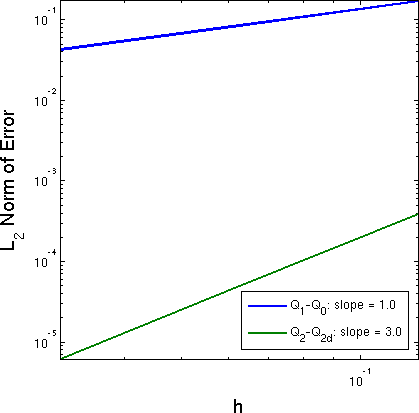
\includegraphics[width=3in,keepaspectratio=true]{./Figures/gp_cp_convQ2Q2.png}
 % elQ1Q0.png: 509x592 pixel, 107dpi, 12.08x14.05 cm, bb=0 0 342 398
 \caption{Convergence of the \el{Q_2}{\hat Q_2} pressure field}
 \label{fig:gp_cp_convQ2Q2}
\end{figure}

\begin{figure}[h!]
 \centering
 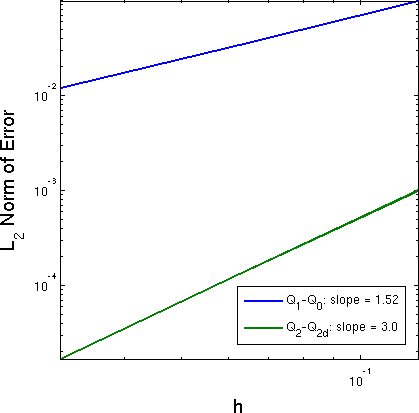
\includegraphics[width=3in,keepaspectratio=true]{./Figures/gp_ca_convQ2Q2.png}
 % elQ1Q0.png: 509x592 pixel, 107dpi, 12.08x14.05 cm, bb=0 0 342 398
 \caption{Convergence of $\Grad p$ acceleration: \el{Q_2}{\hat Q_2} versus \el{Q_1}{Q_1} on a Cartesian mesh}
 \label{fig:gp_ca_convQ2Q2}
\end{figure}

\subsubsection{The $\mathrm{grad}(p)$ Test on a Distorted Mesh}
As we can see from \refFig{gp_da_convQ2Q2}, when we distort the mesh, the convergence rate drops down to 2.9.

\begin{figure}[h!]
 \centering
 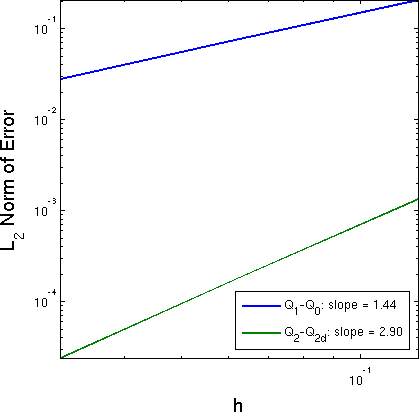
\includegraphics[width=3in,keepaspectratio=true]{./Figures/gp_da_convQ2Q2.png}
 % elQ1Q0.png: 509x592 pixel, 107dpi, 12.08x14.05 cm, bb=0 0 342 398
 \caption{Convergence of $\Grad p$ acceleration: \el{Q_2}{\hat Q_2} versus \el{Q_1}{Q_1} on a distorted mesh}
 \label{fig:gp_da_convQ2Q2}
\end{figure}

\subsubsection{The $\mathrm{div}(\mathrm{grad}(V))$ Test}
This element has the same velocity space as \el{Q_2}{\hat Q_1}, therefore the convergence rates will be identical for the $\mathrm{div}(\mathrm{grad}(V))$ test.

\subsection{Spurious Modes}
This element has some very ugly spurious modes as we see in \refFig{acousticQ2Q2_hgOFF}. During the process of the solution, it appears that the very noisy interior travels outward from the center at half of the wave speed. Thus as the solution progresses, more and more of it will be overcome by the spurious modes.

\begin{figure}[h!]
 \centering
 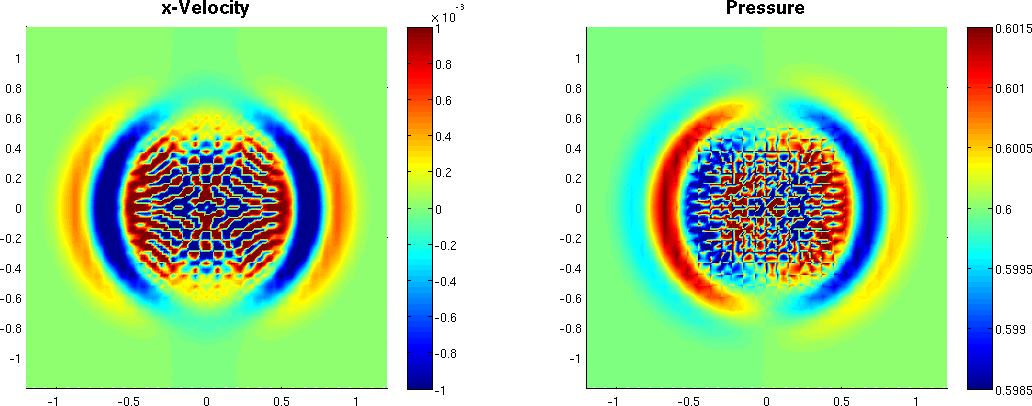
\includegraphics[width=6in,keepaspectratio=true]{./Figures/acousticQ2Q2_hgOFF.png}
 % elQ1Q0.png: 509x592 pixel, 107dpi, 12.08x14.05 cm, bb=0 0 342 398
 \caption{\el{Q_2}{\hat Q_2} acoustic wave without hourglass filter}
 \label{fig:acousticQ2Q2_hgOFF}
\end{figure}

\section{Conclusions}
We have considered a large array of different mixed finite element methods in the course of this research, but it would be prohibitive to attempt to do an in-depth study of every one of these elements for every canonical test problem that we will consider. Thus, we need to pair down the search space to a few mixed finite element pairs that showed the most promise. The \el{Q_1}{\hat Q_1} element has been considered in detail in  \cite{CaramanaShashkov98}, so we will carry the results around for comparison. We would like to focus our study on curvilinear elements because they present a new frontier in the field of Lagrangian hydrodynamics. Therefore we will focus primarily on the \el{Q_2}{\hat Q_1} element, which showed the most promise for a full hydrocode. The \el{Q_2}{\hat P_1} element behaves very similarly, so we can assume that most of the discussion concerning \el{Q_2}{\hat Q_1} will apply to this element as well. We will also consider the \el{Q_2}{\hat Q_2} because it represents the higher order analogue of the method of sub-zonal pressures, namely \el{Q_1}{\hat Q_1}. Of course, we need a control to compare against. With that in mind, we will continue to compare against results from traditional \el{Q_1}{Q_0} SGH with and without hourglass filters.